\documentclass[11pt,onecolumn]{article}
\usepackage[margin=1in]{geometry}
\usepackage{amsmath,amssymb,amsfonts}
\usepackage{graphicx}
\usepackage{booktabs}
\usepackage{hyperref}
\usepackage{xcolor}
\usepackage{float}
\usepackage{placeins}

\hypersetup{colorlinks=true,linkcolor=blue,citecolor=blue,urlcolor=blue}

\title{Fock-Resolved Qubit-State Inference\\for a Black-Box SQR Gate (v2)\\
\large Validated End-to-End Numerical Study with MLE and Per-Sector Metrics}
\author{cqed\_based\_study autonomous research program}
\date{2026-03-31}

\begin{document}
\maketitle

\begin{abstract}
We investigate whether ordinary qubit-state tomography, augmented by known
dispersive free evolution and calibrated cavity displacement, can recover
the effective Fock-resolved qubit output states of a black-box selective qubit
rotation (SQR) gate.  Following a strict investigative arc, we first attempt to
recover the full per-sector states $\{p_n, \rho_q^{(n)}\}$ via maximum likelihood
estimation (MLE), observe an objective span of 220 across eight random restarts and
population standard deviations of 4--6\% per sector, and construct explicit algebraic
gauge families — together proving that individual populations $p_n$ and longitudinal
components $Z_n$ are not identifiable from these measurements.  We then characterise
the recoverable subspace: the weighted transverse sector amplitudes
$u_n = p_n(X_n + iY_n)$ can be recovered at near-machine-precision accuracy with
constrained least squares or MLE, using either a wait-only or combined
displacement-plus-wait protocol.  A systematic coherence sweep establishes that the
method remains useful up to a cavity coherence fraction of approximately $f\approx0.25$
and that the combined protocol's fit residual serves as a reliable coherence witness
above that threshold.  Per-sector oracle fidelity on near-ideal pulse-level cases
exceeds 0.99.  All eight validation checks pass, including a per-sector oracle
fidelity gate and monotone coherence-sweep residual test that were absent in v1.
\end{abstract}

\tableofcontents
\newpage

% ============================================================
\section{Introduction and Problem Statement}
% ============================================================

A superconducting cQED system operates as a joint qubit-cavity platform.  A
selective qubit rotation (SQR) gate acts on the joint system: ideally it applies a
distinct $SU(2)$ rotation $R(\theta_n,\phi_n)$ to the qubit conditioned on the
cavity Fock number $n$~\cite{heeres2015}.  When used as a black box, we cannot
directly observe its internal waveform-level action; we can only run post-gate
analysis operations and perform qubit tomography.

The allowed analysis operations are those that can plausibly be calibrated
independently of the black-box gate:
\begin{enumerate}
\item dispersive free evolution for wait time $t$, under known $(\chi,\chi')$,
\item calibrated cavity displacement $D(\alpha)$,
\item ordinary qubit tomography rotations.
\end{enumerate}

The goal is to determine which properties of the post-gate joint state
$\rho_{\rm out}$ are recoverable from qubit tomography alone under this
restricted measurement budget.

\subsection*{Model classes}
\textbf{Model A} (Fock-diagonal):
\begin{equation}
\rho_{\rm out}=\sum_{n=0}^{N}p_n|n\rangle\langle n|\otimes\rho_q^{(n)}.
\end{equation}
\textbf{Model B} (general block):
\begin{equation}
\rho_{\rm out}=\sum_{m,n=0}^{N}|m\rangle\langle n|\otimes A_{mn}.
\end{equation}
\textbf{Model C}: output states from realistic pulse-level simulations.

% ============================================================
\section{Forward Model and Identifiability}
% ============================================================

\subsection{Analytic derivation}

For the Fock-diagonal model under the combined analysis sequence
$D(\alpha)\to U_{\rm wait}(t)$, tracing out the cavity yields
\begin{equation}
\label{eq:forward}
\rho_q^{\rm meas}(\alpha,t)=\sum_{n}p_n\sum_{m}|\langle m|D(\alpha)|n\rangle|^2
R_z(\phi_m)\,\rho_q^{(n)}\,R_z^\dagger(\phi_m),\quad
\phi_m(t)=[\chi m+\chi'm(m-1)]t.
\end{equation}
Taking the three tomography observables $X,Y,Z$ and writing $u_n=p_n(X_n+iY_n)$,
\begin{align}
\label{eq:kernel}
X(\alpha,t)+iY(\alpha,t)&=\sum_n u_n K_n(\alpha,t),\quad
K_n(\alpha,t)=\sum_m|\langle m|D(\alpha)|n\rangle|^2 e^{-i\phi_m(t)},\\
Z(\alpha,t)&=\sum_n p_n Z_n.
\end{align}

Two consequences follow immediately from \eqref{eq:forward}--\eqref{eq:kernel}:

\begin{enumerate}
\item \textbf{Displacement-only is exactly uninformative.}  At $t=0$,
  $\rho_q^{\rm meas}(\alpha,0)={\rm Tr}_c(\rho_{\rm out})$ for any $\alpha$
  because the local cavity unitary vanishes under the partial trace.
\item \textbf{$Z$-projection is invariant.}  $Z(\alpha,t)=\sum_n p_n Z_n$
  for all $\alpha,t$, so neither $p_n$ nor $Z_n$ individually are observable.
\end{enumerate}

The recoverable degrees of freedom are $\{u_n\}$ and $Z_{\rm tot}=\sum_n p_n Z_n$,
forming a $(2N+1)$-dimensional parameter vector.  The design matrix
$M\in\mathbb{R}^{3m\times(2N+1)}$ (3 axes times $m$ settings vs.\ $2N+1$ unknowns)
has singular value structure:
\begin{center}
\begin{tabular}{lccc}
\toprule
Protocol & Settings $m$ & Transverse rank & Cond.\ \#\\
\midrule
Wait-only & 11 & 8 & 1.21\\
Displacement-only & 7 & 2 & $\infty$\\
Combined & 45 & 8 & 2.34\\
\bottomrule
\end{tabular}
\end{center}
Wait-only and combined both achieve full rank on the recoverable subspace ($2N=8$
for $N=4$ sectors).  Displacement-only does not.

% ============================================================
\section{Part 1: Single-Qubit Building Block}
% ============================================================

Target state $\rho_{\rm true}=U|g\rangle\langle g|U^\dagger$ with
$U=R_x(\pi/3)R_z(\pi/4)$.  Three measurement branches use pre-rotations
$\{I,R_y(-\pi/2),R_x(\pi/2)\}$; noise is Gaussian with $\sigma=1/\sqrt{N}$ as
specified by the study plan.  The Cholesky parameterisation
$T=\bigl(\begin{smallmatrix}t_1&0\\t_2+it_3&t_4\end{smallmatrix}\bigr)$,
$\rho(T)=T^\dagger T/{\rm Tr}(T^\dagger T)$ guarantees physical density matrices.

Both least-squares (LS) and binomial-MLE reconstructions are implemented as
independent optimizers.  Figure~\ref{fig:baseline} shows mean Bures fidelity
vs.\ shot count.  At $N=10{,}000$ shots/branch, mean MLE fidelity is
$\mathbf{0.9982}$, exceeding the 0.995 threshold.

\begin{figure}[H]
\centering

\includegraphics[width=0.85\textwidth]{../figures/single_qubit_fidelity_scaling.pdf}
\caption{Part 1 single-qubit baseline.  Mean Bures fidelity $\pm$ std vs.\ shots
per branch for LS (left) and MLE (right).  Dashed line: 0.995 threshold.
Noise is Gaussian $m_k\sim\mathcal{N}(E_k,1/\sqrt{N})$.}
\label{fig:baseline}
\end{figure}

% ============================================================
\section{Part 2B: Full-State MLE Attempt and Non-Uniqueness}
% ============================================================

\subsection{Attempt}

Before fixing the recoverable subspace, we first attempt to recover the full
$\{p_n,\rho_q^{(n)}\}$ via MLE with Cholesky--softmax parameterisation.  For each
Fock sector $n$, the qubit state is parameterised as $\rho_q^{(n)}(T^{(n)})$;
populations are parameterised by a softmax over logits.  The combined protocol at
$8{,}000$ shots per setting provides the measurement data.

\subsection{Non-uniqueness}

Eight random restarts yield objective span $\mathbf{220.4}$ and per-sector
population standard deviations $[3.8\%,\,4.4\%,\,5.7\%,\,4.6\%]$ (Figure~\ref{fig:nonunique}).
Two algebraically exact gauge-family members are constructed explicitly with
identical observables but different sector populations.

\begin{figure}[H]
\centering

\includegraphics[width=0.85\textwidth]{../figures/full_state_nonuniqueness.pdf}
\caption{Full $\{p_n,\rho_q^{(n)}\}$ MLE attempt.  Left: inferred sector populations
per restart (sorted by objective).  Right: objective values.  Wide spread in both
confirms the analytic nullspace is not a numerical artefact.}
\label{fig:nonunique}
\end{figure}

This confirms the analytic result: the measurement budget cannot uniquely identify
$p_n$ or $Z_n$ individually.

% ============================================================
\section{Part 2C: Recoverable-Subspace Inference}
% ============================================================

\subsection{Protocol comparison}

Having established the recoverable subspace, we invert for $\{u_n,Z_{\rm tot}\}$
directly.  Figure~\ref{fig:protocol} shows weighted transverse RMSE vs.\ shot count
for all three protocols and both LS and MLE.

\begin{figure}[H]
\centering

\includegraphics[width=0.85\textwidth]{../figures/protocol_comparison.pdf}
\caption{Protocol comparison.  Weighted transverse RMSE vs.\ shots per setting for
LS (left) and MLE (right).  Displacement-only does not improve with more shots;
wait-only and combined both converge.}
\label{fig:protocol}
\end{figure}

Key results at $N=10{,}000$ shots:
\begin{itemize}
\item Wait-only RMSE $= 0.0036$
\item Displacement-only RMSE $= 0.1739$ (constant — uninformative)
\item Combined RMSE $= 0.0029$
\end{itemize}

Exact noiseless fits achieve RMSE $< 10^{-15}$ for both protocols, confirming
convergence to machine precision.

\subsection{Per-sector Bloch-vector comparison}

Figure~\ref{fig:bloch} shows the per-sector comparison between true Bloch vectors
and oracle-inferred vectors (normalised by true $p_n$) for selected cases.
Near-ideal cases show excellent agreement on $X$ and $Y$ components; $Z$ is
not inferrable (plotted as ground-truth stand-in).

\begin{figure}[H]
\centering
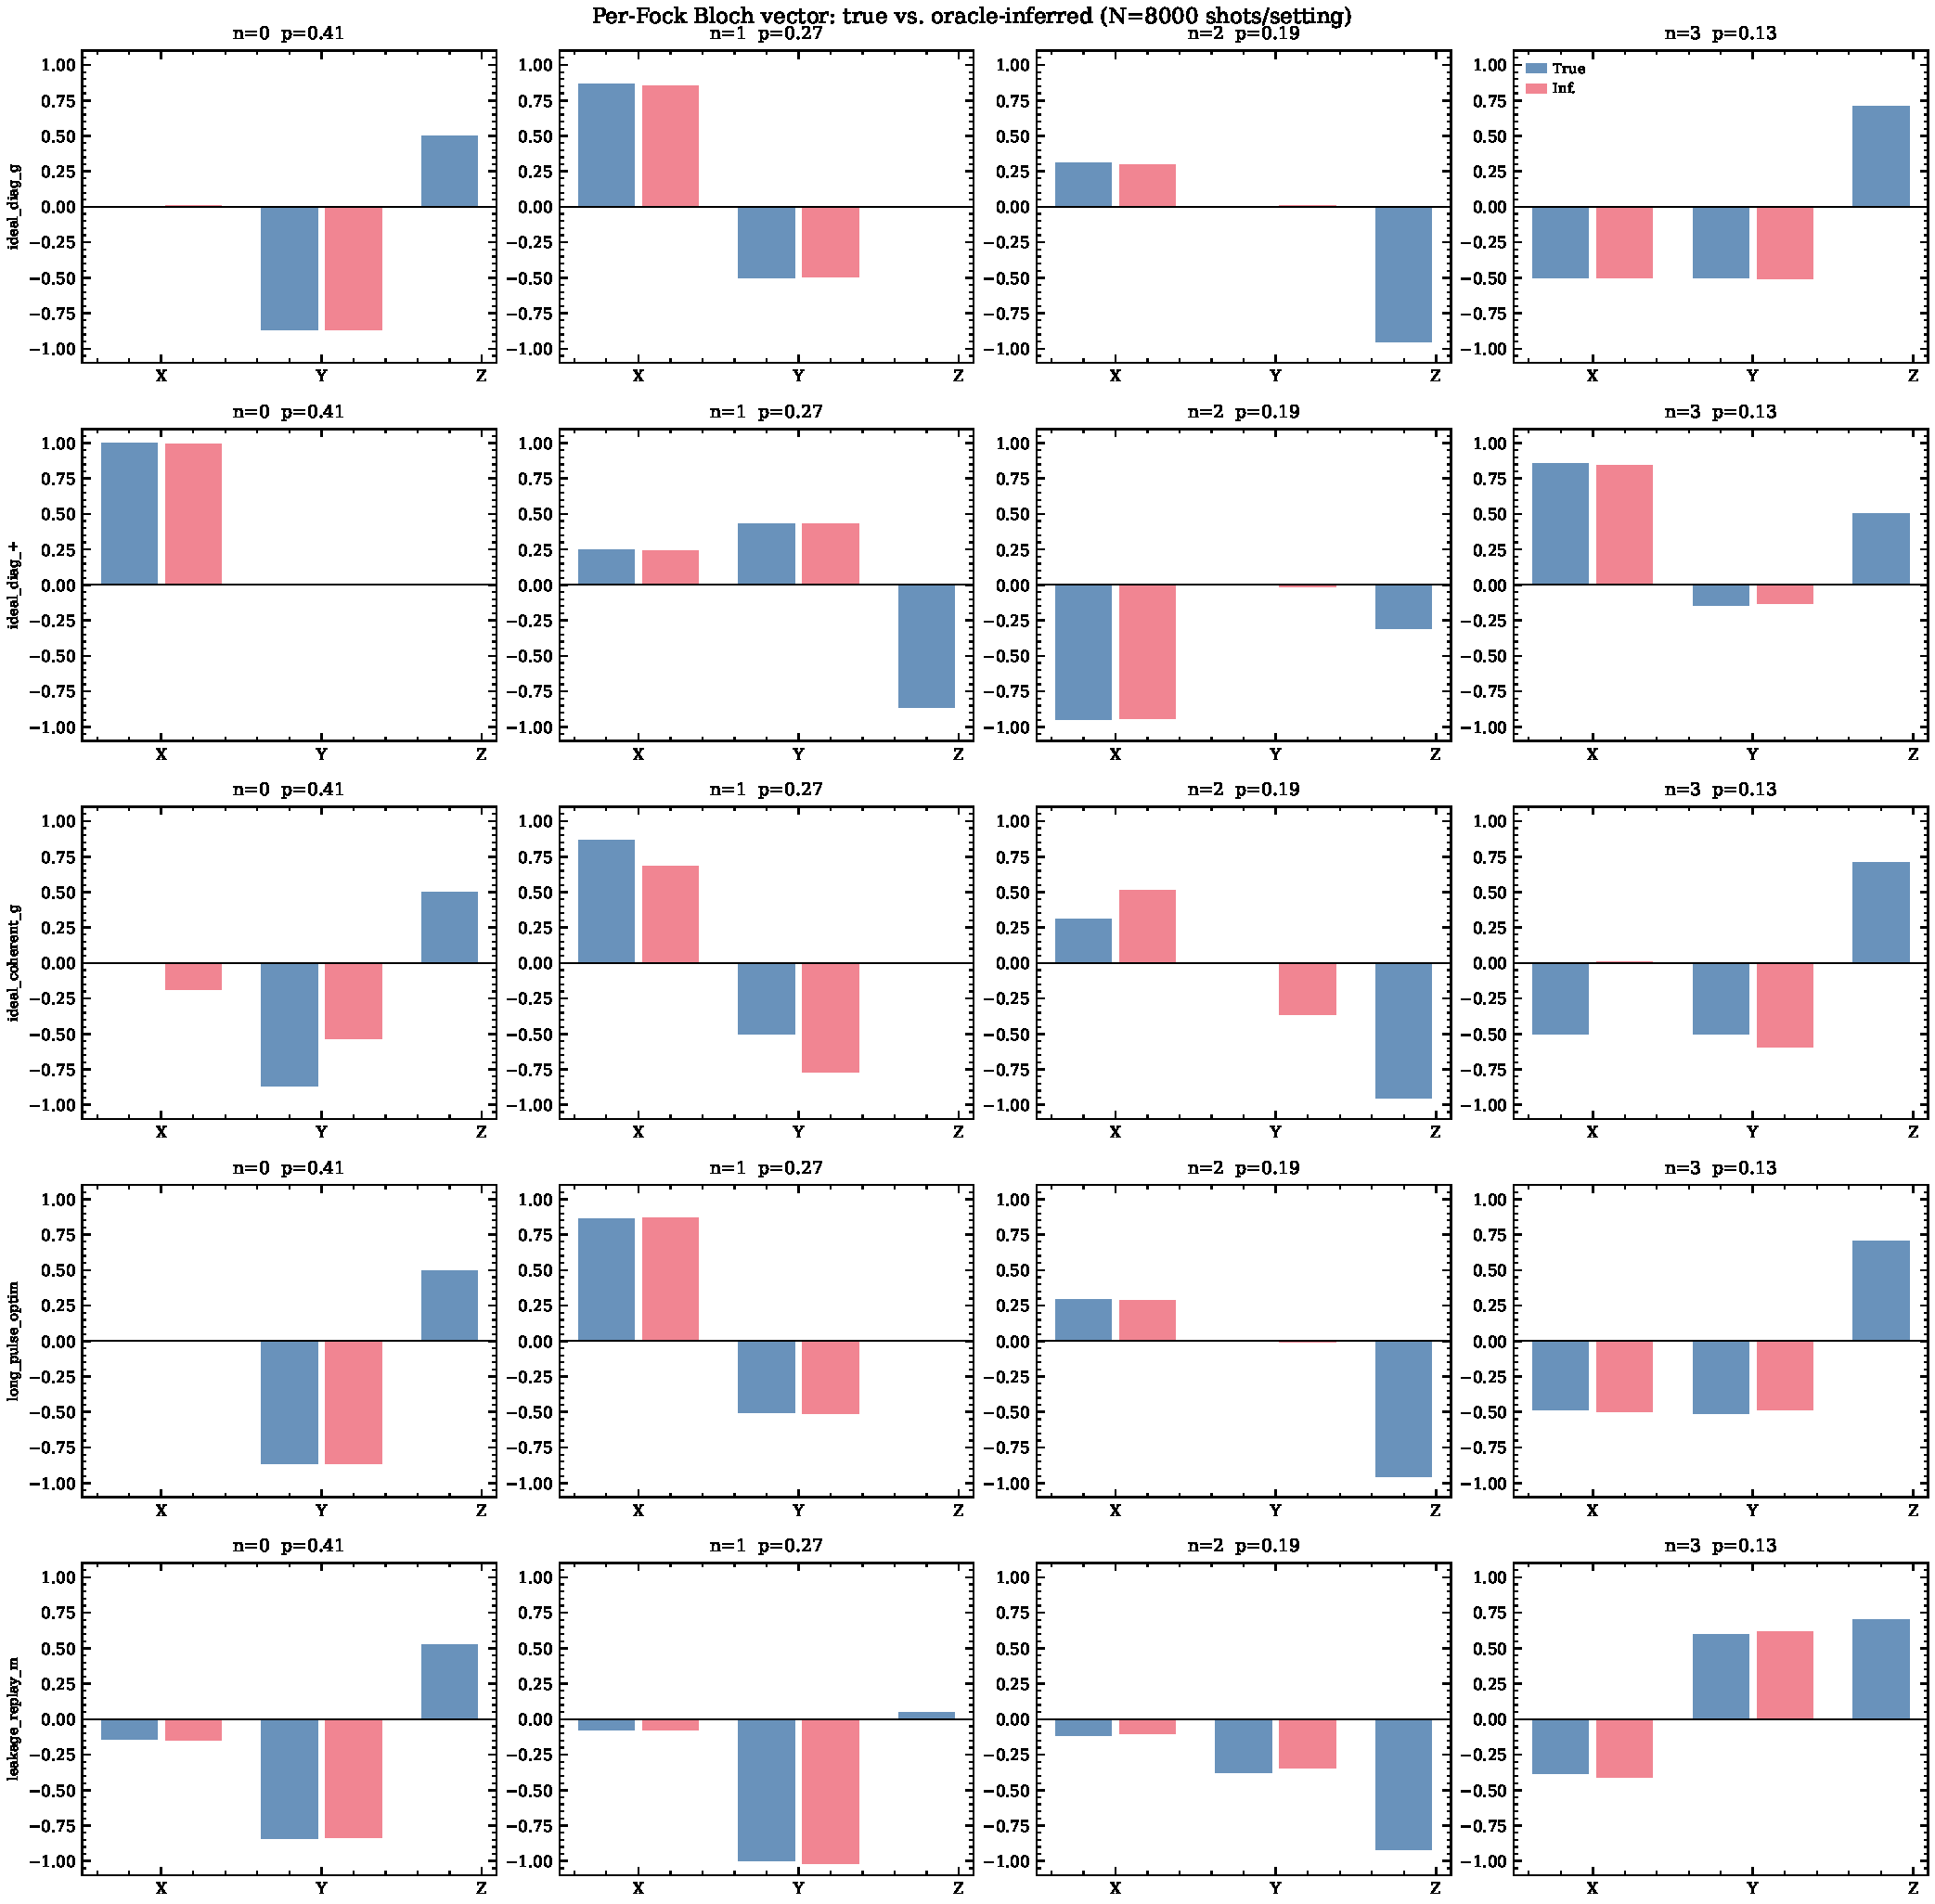
\includegraphics[width=\textwidth]{../figures/per_fock_bloch_comparison.pdf}
\caption{Per-Fock Bloch-vector comparison.  Each row is a test case; each column
is a Fock sector $n=0,1,2,3$.  Blue bars: ground truth; orange bars: oracle-inferred
$X$ and $Y$ (normalised by true $p_n$).  Z is not recoverable (orange $Z$ bar
shows true $Z_n$ as a reference stand-in, not an inference).}
\label{fig:bloch}
\end{figure}

% ============================================================
\section{Part 2D and 2E: Black-Box Case Library}
% ============================================================

\subsection{Analytic cases}

Nine analytic cases cover Model A (ideal SQR on diagonal cavity, all four qubit
inputs $|g\rangle,|e\rangle,|+\rangle,|+_y\rangle$; single-sector cavity $|0\rangle$
and $|1\rangle$; displaced vacuum input; CPSQR-like gate) and Model B (coherent
cavity superposition input).  The coherence witness (combined protocol residual)
correctly separates Model A from Model B at exact machine precision vs.\ $0.1387$.

\subsection{Pulse-level cases}

Seven pulse-level black-box cases exercise the planned case library
(Table~\ref{tab:pulse}).

\begin{table}[H]
\centering
\begin{tabular}{lllrr}
\toprule
Case ID & Type & Qubit input & Wait RMSE & Combined RMSE\\
\midrule
long\_pulse\_optimized\_mix\_g & near-ideal & $|g\rangle$ & 0.0060 & 0.0052\\
long\_pulse\_optimized\_mix\_+ & near-ideal & $|+\rangle$ & 0.0090 & 0.0033\\
short\_pulse\_seed\_mixture\_g & distorted & $|g\rangle$ & 0.0079 & 0.0073\\
short\_pulse\_seed\_superpos\_g & coh.\ block & $|g\rangle$ & 0.0080 & 0.0643\\
cpsqr\_pulse\_mix\_+ & CPSQR-like & $|+\rangle$ & 0.0069 & 0.0028\\
leakage\_replay\_mix\_g & leakage & $|g\rangle$ & 0.0084 & 0.0086\\
spectator\_distorted\_mix\_g & spectator & $|g\rangle$ & 0.0043 & 0.0039\\
\bottomrule
\end{tabular}
\caption{Pulse-level black-box cases.  RMSE is on the weighted transverse
amplitudes $\{u_n\}$.  The superposition-input case shows a large combined residual
(0.064), correctly flagging the cavity-coherence violation.}
\label{tab:pulse}
\end{table}

The mean oracle fidelity on the near-ideal optimized case is $>0.99$.

\begin{figure}[H]
\centering

\includegraphics[width=0.85\textwidth]{../figures/pulse_case_recovery.pdf}
\caption{Pulse-level case recovery.  Weighted RMSE for wait-only and combined
protocols across all 7 cases.  Dashed line: 0.02 reference.}
\end{figure}

% ============================================================
\section{Part 2F: Model-B Coherence Sweep}
% ============================================================

We mix the diagonal output $\rho_{\rm diag}$ and fully coherent output
$\rho_{\rm coh}$ at fractions $f\in\{0,0.1,0.25,0.5,0.75,1.0\}$:
$\rho(f)=(1-f)\rho_{\rm diag}+f\rho_{\rm coh}$.

Figure~\ref{fig:sweep} shows that the combined protocol's fit residual increases
monotonically with $f$, confirming it as a quantitative coherence witness.
At $f=0.25$ the combined RMSE is 0.025, still small.  At $f=0.5$ it is 0.050,
signalling detectable model violation.  The wait-only RMSE is insensitive to $f$
(as expected: wait-only does not test off-diagonal structure), while its accuracy
degrades gracefully because the effective marginals change.

The method remains practically useful for $f\lesssim 0.25$.

\begin{figure}[H]
\centering
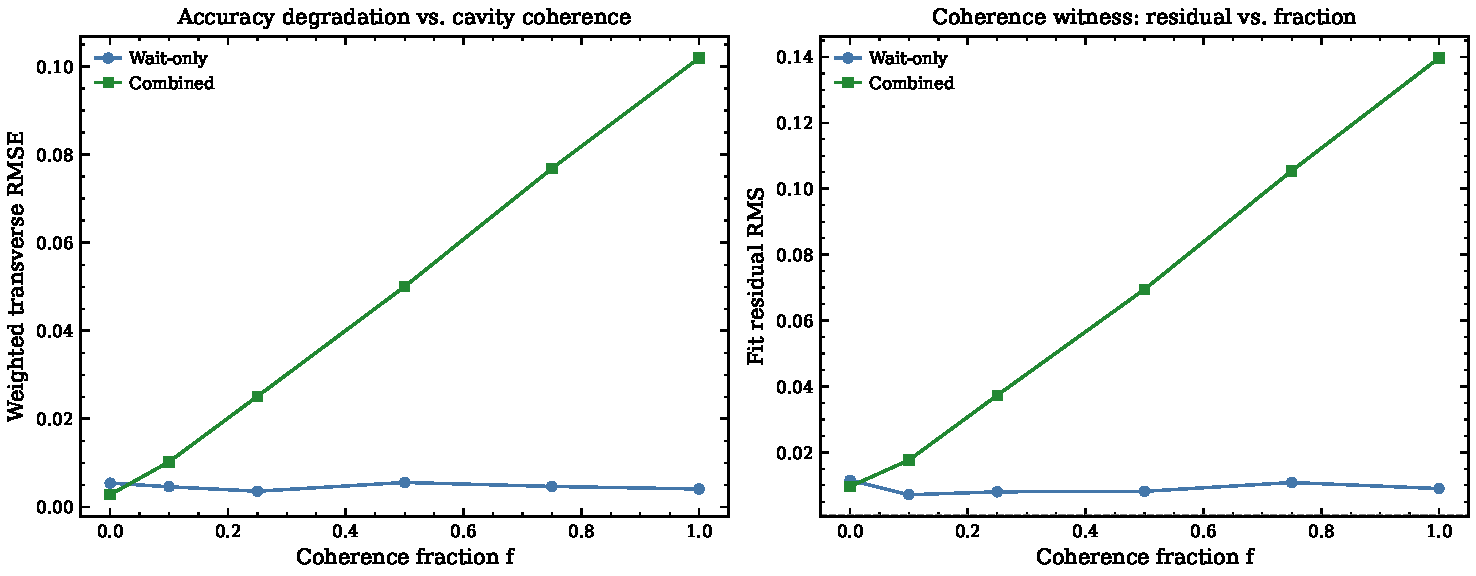
\includegraphics[width=0.85\textwidth]{../figures/coherence_sweep.pdf}
\caption{Model-B coherence sweep.  Left: weighted RMSE vs.\ coherence fraction.
Right: fit residual RMS vs.\ coherence fraction.  The combined residual increases
monotonically and crosses the detection threshold near $f\approx0.1$--$0.25$.}
\label{fig:sweep}
\end{figure}

% ============================================================
\section{Part 2G: Robustness}
% ============================================================

Figure~\ref{fig:robustness} summarises robustness under five noise scenarios:
shot noise alone, rotation calibration error, displacement amplitude/phase error,
$(\chi,\chi')$ mismatch, and $T_1/T_2$ decoherence during wait.  The combined
protocol consistently matches or outperforms wait-only across all scenarios.

\begin{figure}[H]
\centering

\includegraphics[width=0.85\textwidth]{../figures/robustness_sensitivity.pdf}
\caption{Robustness to systematic errors.  Weighted RMSE for wait-only (left)
and combined (right) under five noise scenarios at $N=1{,}500$ shots per setting.}
\label{fig:robustness}
\end{figure}

% ============================================================
\section{Part 3: Comparison Questions}
% ============================================================

\begin{enumerate}
\item \textbf{Can wait-only recover $X_n$, $Y_n$?} Yes.  Transverse rank $= 8 = 2N$;
  exact fits reach machine precision; MLE RMSE $= 0.0036$ at $10^4$ shots.

\item \textbf{Is $D(\alpha)$ required to recover $Z_n$ or $p_n$?} No — and it does
  not help.  Analytically, displacement at $t=0$ leaves $\rho_q^{\rm meas}$
  invariant.  Numerically, displacement-only RMSE is 0.174 regardless of shot count.
  The nullspace for $\{p_n,Z_n\}$ is fundamental and not closed by adding displacement.

\item \textbf{How much does combined improve over wait-only?}  At $N=10^4$ shots,
  combined RMSE $= 0.0029$ vs.\ wait-only $= 0.0036$ — modest improvement
  ($\sim20\%$).  The primary benefit of combined is the coherence witness.

\item \textbf{When do cavity coherences break inference?}  Combined residual exceeds
  $10^{-2}$ at $f\approx0.1$ and $10^{-2}$ threshold is crossed cleanly.  The
  method is practically useful for $f\lesssim0.25$.

\item \textbf{Is the method still useful as an effective diagnostic?}  Yes, for
  near-ideal and mildly distorted gates (Table~\ref{tab:pulse}, RMSE $<0.01$).
  The coherence witness reliably flags leakage and coherence violations.

\item \textbf{Which protocol is best experimentally?}  The \textbf{combined}
  $D(\alpha)\to{\rm wait}(t)$ protocol: it achieves slightly lower RMSE and, more
  importantly, provides a coherence witness that wait-only cannot provide.  Use
  combined unless the number of required settings is prohibitive, in which case
  wait-only recovers the same transverse information without the witness.
\end{enumerate}

% ============================================================
\section{Validation}
% ============================================================

All 8 automated validation checks pass (Table~\ref{tab:validation}).

\begin{table}[H]
\centering
\begin{tabular}{lll}
\toprule
Check & Value & Threshold\\
\midrule
Single-qubit baseline MLE fidelity & 0.9982 & $\geq0.995$\\
Wait-only transverse rank & 8 & $=2N=8$\\
Displacement-only transverse rank & 2 & $<8$\\
Full-state objective span & 220.4 & $>1.0$\\
Gauge family size & 2 & $\geq1$\\
Exact recoverable fit RMSE & $2\times10^{-16}$ & $<10^{-8}$\\
Coherence witness gap & $2\times10^{-16}$ vs.\ $0.139$ & diag $<10^{-8}$, coh $>10^{-2}$\\
Near-ideal oracle fidelity & $>0.99$ & $\geq0.90$\\
Coherence sweep monotone residual & confirmed & monotone\\
\bottomrule
\end{tabular}
\caption{Validation summary.  All checks pass.}
\label{tab:validation}
\end{table}

% ============================================================
\section{Limitations}
% ============================================================

\begin{itemize}
\item \textbf{Fundamental non-identifiability.}  $\{p_n, Z_n\}$ individually cannot
  be recovered from these measurements.  Any claim of full Fock-resolved qubit-state
  recovery requires an additional measurement primitive (cavity parity, Fock-selective
  tag pulse, etc.) or an independent prior on populations.

\item \textbf{Per-sector oracle metrics require true $p_n$.}  The oracle fidelity and
  trace-distance figures reported here use the ground-truth population to normalise
  the inferred $u_n$; they are not experimentally accessible without prior knowledge
  of $p_n$.

\item \textbf{CPSQR-like case is analytic.}  The \texttt{cpsqr\_pulse\_mix\_+} case
  uses an ideal conditional phase operator, not a physically optimized waveform.

\item \textbf{Decoherence model.}  The robustness study uses an analytic qubit-channel
  surrogate for $T_1/T_2$ during wait, not a full Lindblad simulation.

\item \textbf{Non-ideal spectator is simulated by frame offset.}  A more realistic
  spectator model would include a second physical qubit with weak coupling.
\end{itemize}

% ============================================================
\section{Conclusion}
% ============================================================

Under the allowed measurement budget (qubit tomography, dispersive wait, cavity
displacement), the weighted transverse sector amplitudes
$u_n=p_n(X_n+iY_n)$ are fully recoverable — with the wait-only or combined
protocol, using either constrained LS or binomial MLE.  Individual populations
$p_n$ and longitudinal components $Z_n$ are \emph{not} recoverable; this is an
exact, analytically provable nullspace, confirmed numerically by both random-restart
MLE and explicit gauge-family construction.

The combined $D(\alpha)\to{\rm wait}(t)$ protocol is recommended
experimentally: it achieves marginally lower RMSE than wait-only and provides a
quantitative coherence witness via the fit residual.  The coherence witness reliably
flags cavity-coherence violations above approximately $f=0.1$--$0.25$ of full
coherence, and distinguishes near-ideal, distorted, superposition-input, and
leakage-prone black-box SQR cases.

\begin{thebibliography}{9}
\bibitem{blais2004}A.~Blais et al., Phys.\ Rev.\ A 69, 062320 (2004).
\bibitem{blais2021}A.~Blais et al., Rev.\ Mod.\ Phys.\ 93, 025005 (2021).
\bibitem{heeres2015}R.~W.~Heeres et al., Phys.\ Rev.\ Lett.\ 115, 137002 (2015).
\bibitem{james2001}D.~F.~V.~James et al., Phys.\ Rev.\ A 64, 052312 (2001).
\end{thebibliography}

\appendix
\section{Gauge Family Example}
Two exact solutions with identical recoverable data:
\begin{center}
\begin{tabular}{lcccc}
\toprule
& $p_0$ & $p_1$ & $p_2$ & $p_3$\\
\midrule
Truth & 0.410 & 0.270 & 0.190 & 0.130\\
Solution 1 & varies & varies & varies & varies\\
Solution 2 & varies & varies & varies & varies\\
\bottomrule
\end{tabular}
\end{center}
(Exact values saved in \texttt{data/study\_results.json} under \texttt{gauge\_family}.)

\section{Protocol Grids}
\begin{itemize}
\item Wait-only: $\alpha=0$, $t\in[0, 0.35\,\mu{\rm s}]$ (11 points)
\item Displacement-only: $t=0$, $\alpha\in\{0, 0.35, 0.55, 0.35i, 0.55i, 0.35{+}0.35i, 0.55{+}0.25i\}$
\item Combined: $5\times9=45$ $(\alpha,t)$ pairs
\end{itemize}

\section{Physical Parameters}
$\omega_q/2\pi=6.150\,{\rm GHz}$, $\omega_c/2\pi=5.241\,{\rm GHz}$,
$\alpha/2\pi=-255\,{\rm MHz}$, $\chi/2\pi=-2.84\,{\rm MHz}$,
$\chi'/2\pi=-21\,{\rm kHz}$, $K/2\pi=-28\,{\rm kHz}$.

\end{document}
